\documentclass[utf8,xcolor=table]{beamer}

\usepackage[T2A]{fontenc}
\usepackage[utf8]{inputenc}
\usepackage[english,russian]{babel}
\usepackage{tikz}
\usetikzlibrary{shapes,arrows}
\usepackage{dot2texi}
\usepackage{minted}
\usepackage{ulem}
\usepackage{cmap}
\usepackage{multirow}

\hypersetup{colorlinks,linkcolor=blue,urlcolor=blue}

\mode<presentation>{
	\usetheme{CambridgeUS}
}

\renewcommand{\t}[1]{\ifmmode{\mathtt{#1}}\else{\texttt{#1}}\fi}

\title{Типы в Haskell}
\author{Егор Суворов}
\institute[СПбГУ]{Курс <<Парадигмы и языки программирования>>, группа 18.Б09-пу}
\date[24.04.2019]{Среда, 24 апреля 2019 года}

\setlength{\arrayrulewidth}{1pt}

\begin{document}

\begin{frame}
\titlepage
\end{frame}

\begin{frame}{План занятия}
	\tableofcontents
\end{frame}

\section{Ещё про Haskell}
\subsection{Функции высшего порядка}

\begin{frame}
	\tableofcontents[currentsection,currentsubsection]
\end{frame}

\begin{frame}{Напоминание}
	\begin{itemize}
		\item Функция является \textit{функцией высшего порядка}, если она в качестве одного из аргументов принимает другую функцию.
		\item Пример: \t{map}. Он первым параметром принимает функцию, которая преобразует элементы списка.
		\item Функции высшего порядка является основными кирпичиками в функциональном программировании.
	\end{itemize}
\end{frame}

\begin{frame}[fragile]{Ещё один паттерн}
\begin{minted}{haskell}
sum (x:xs) = x + sum xs
sum _ = 0

prod (x:xs) = x * prod xs
prod _ = 1

max (x:xs) = max x (max xs)
max x = -1

concat (x:xs) = x ++ (concat xs)
concat _ = ""
\end{minted}
	Что общего?
	\pause
	\begin{itemize}
		\item Все эти функции считают функцию от множества элементов.
		\item Для пересчёта требуется знать только текущее значение и очередной элемент.
	\end{itemize}
\end{frame}

\begin{frame}[t,fragile]{Правая свёртка}
\begin{minted}{haskell}
foldr f a (x:xs) = f x (foldr f a xs)
foldr f a _ = a

sum    xs = foldr (+)  0    xs
prod   xs = foldr (*)  1    xs
max    xs = foldr max  (-1) xs
concat xs = foldr (++) ""   xs
\end{minted}
	Ещё одна популярная функция высшего порядка.
\end{frame}

\begin{frame}[fragile]{Упражнение на понимание}
\begin{minted}{haskell}
foldr f a (x:xs) = f x (foldr f a xs)
foldr f a _ = a
\end{minted}

	А что такое \t{foldr (:) [4,5] xs}?
	\pause
\begin{minted}{haskell}
foldr (:) [4,5] [1,2,3] =
1:(foldr (:) [4,5] [2,3]) =
1:(2:(foldr (:) [4,5] [3])) =
1:(2:(3:(foldr (:) [4,5] []))) =
1:(2:(3:[4,5])) =
[1,2,3,4,5]
\end{minted}
	Дописывание \t{[4,5]} в конец списка.

\begin{minted}{haskell}
(++) a b = foldr (:) b a
\end{minted}
\end{frame}

\begin{frame}{Картинка}
	\begin{center}
		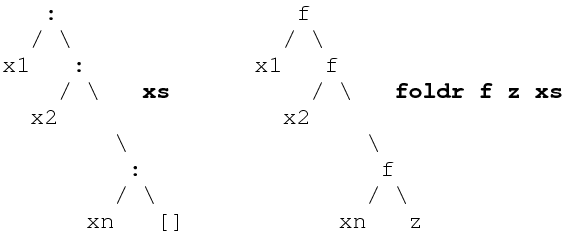
\includegraphics[scale=0.5]{foldr.png}
	\end{center}
	Бамбук растёт вправо, поэтому \textit{правая} свёртка.
\end{frame}

\begin{frame}[fragile]{Упражнения}
	Как узнать, все ли элементы равны \t{True}? \pause
\begin{minted}{haskell}
foldr (&&) True xs
\end{minted}

	Как узнать сумму квадратов чисел в массиве? \pause
\begin{minted}{haskell}
foldr (+) 0 (map (^2) xs)
\end{minted}

	Как выразить \t{map} через \t{foldr}? \pause
\begin{minted}{haskell}
map f xs = foldr (\a x -> (f a):x) [] xs
\end{minted}
	Вывод: в теории почти всё есть \t{foldr}.
	На практике лучше использовать готовые функции.
\end{frame}

\subsection{Мемоизация}

\begin{frame}
	\tableofcontents[currentsection,currentsubsection]
\end{frame}

\begin{frame}[t,fragile]{Ленивые числа Фибоначчи}
\begin{minted}{haskell}
fib 0 = 0
fib 1 = 1
fib n = fib (n - 2) + fib (n - 1)
\end{minted}
	\t{fib 100} работает бесконечно долго.
	Несмотря на то, что \t{fib 10} можно запомнить,
	Haskell не запоминает вообще все вычисления функций в программе
	(а программа "--- это одно большое вычисление).

	Можно обхитрить ленивыми списками:
\begin{minted}{haskell}
fibs = map fib' [0..]
    where
        fib' 0 = 0
        fib' 1 = 1
        fib' n = fibs !! (n - 1) + fibs !! (n - 2)
\end{minted}
	Теперь у нас есть одно ленивое значение (\t{fibs}), которое Haskell
	постоянно помнит.
\end{frame}

\begin{frame}[t,fragile]{Сокращаем код}
	Можно записать даже вот так:
\begin{minted}{haskell}
fib = (map fib' [0..] !!)
    where
        fib' 0 = 0
        fib' 1 = 1
        fib' n = fib (n - 1) + fib (n - 2)
\end{minted}

	А вот так уже не катит:
\begin{minted}{haskell}
fib n = map fib' [0..] !! n
    where
       ...
\end{minted}
	
	Вроде бы\footnote{\href{https://stackoverflow.com/a/3951092/767632}{stackoverflow.com/a/3951092/767632}}
	Haskell вычисляет выражение не больше одного раза \textit{внутри одного вызова лямбда-функции}.
\begin{minted}{haskell}
fib = \n -> map fib' [0..] !! n
\end{minted}
\end{frame}

\section{Алгебраические типы данных}
\subsection{Откуда берётся тип-сумма}

\begin{frame}
	\tableofcontents[currentsection,currentsubsection]
\end{frame}

\begin{frame}{Упражнение}
	\begin{itemize}
		\item Пусть у интернет-магазина есть три способа оплаты:
			\begin{enumerate}
				\item Банковской картой, нужно знать её данные.
				\item Наличными при получении, ничего дополнительно знать не нужно.
				\item Выставление счёта на QIWI-кошелёк, нужно знать номер телефона.
			\end{enumerate}
		\item Требуется создать тип данных <<способ оплаты>>, который можно хранить и обрабатывать.
		\item Иногда требуется преобразовывать способ оплаты в строку.
		\item Иногда требуется понимать, надо ли что-то делать с сервере для проведения оплаты (если да "--- положить в очередь).
	\end{itemize}
\end{frame}

\begin{frame}[fragile]{Упражнение (C-подход)}
\begin{minted}{cpp}
enum PaymentMethodType { CARD, CASH, QIWI_BILL };
struct PaymentMethod {
  PaymentMethodType type;
  CardInfo card_info;
  char phone[20];
};
\end{minted}
	\begin{itemize}
		\item Надо везде явно смотреть на поле \t{type} и городить if'ы.
		\item Для обработки пишем функции вроде \t{to\_string}, которые разбирают случаи.
		\item Можем случайно обратиться к \t{card\_info}, если не проверим способ оплаты.
		\item Храним больше байт, чем реально надо (можно \t{union}, но там есть свои проблемы).
	\end{itemize}
\end{frame}

\begin{frame}{Упражнение (ООП-подход)}
	\begin{itemize}
		\item Вводим интерфейс \t{PaymentMethod}, а сами методы делаем подклассами.
		\item Общие функции вроде \t{to\_string} вносим в интерфейс.
		\item Специфичные функции либо руками разбирают случаи, либо используют Visitor.
		\item Так обычно и делают.
		\item Можно добавлять как новые классы, так и новые операции с объектами.
	\end{itemize}
\end{frame}

\subsection{Что такое тип-сумма}
\begin{frame}[fragile]{Тип-сумма}
	\begin{itemize}
		\item Можно ввести \textit{тип-сумму}: множество его допустимых значений равно \textit{дизъюнктному объединению}\footnote{объединение попарно непересекающихся множеств} допустимых значений составных частей.
		\item Чтобы обобщить до суммы произвольных типов, можно каждому значению составной части добавить <<тэг>>.
		\item Пример: тип <<способ оплаты>>:
\begin{minted}{haskell}
data PaymentMethod = BankCard String | Cash | Qiwi String
a = BankCard "1234 5678 9012 3456"
b = Cash
c = Qiwi "+7 812 000 00 00"
\end{minted}
		\item Обычно встречается в функциональных языках.
		\item Именно его наличие обычно подразумевают под <<наличием алгебраических типов данных>>.
	\end{itemize}
\end{frame}

\begin{frame}[fragile]{Тип-сумма: подробности}
\begin{minted}{haskell}
data PaymentMethod = BankCard String | Cash | Qiwi String
\end{minted}
	\begin{itemize}
		\item \t{PaymentMethod} называется \textit{конструктором типа}.
		\item \t{BankCard}, \t{Cash}, \t{Qiwi} называются <<конструкторами данных>>, являются теми самыми <<тэгами>>.
		\item Не путать с конструкторами в ООП!
		\item И конструктор типа, и конструктор данных долнжы начинаться с большой буквы.
		\item Работает с pattern matching:
\begin{minted}{haskell}
to_string (BankCard num) = "BankCard " ++ num
to_string Cash           = "Cash"
to_string (Qiwi phone)   = "Qiwi " ++ phone
\end{minted}
		\item Можно дописать в конец строки с \t{data} слова \t{deriving Show}, чтобы GHCI мог выводить значения типа \t{PaymentMethod}.
	\end{itemize}
\end{frame}

\subsection{Примеры типов-сумм}
\begin{frame}
	\tableofcontents[currentsection,currentsubsection]
\end{frame}

\begin{frame}[fragile]{CharOrNotFound}
	Поиск элемента по номеру:
\begin{minted}{haskell}
data CharOrNotFound = NotFound | Found Char deriving Show

getItem :: [Char] -> Int -> CharOrNotFound
getItem (x:_ ) 0         = Found x
getItem (x:xs) n | n > 0 = getItem xs (n - 1)
getItem _      _         = NotFound
\end{minted}
	\begin{itemize}
		\item Не требуются <<магические значения>> для ситуации <<элемент не найден>>.
		\item Компилятор проверяют, что мы всегда обрабатываем оба случая (\t{ghci~-W~file.hs}).
		\item По типу функции сразу понятно, что она может вернуть.
		\item Нет исключений; функции чистые.
	\end{itemize}	
\end{frame}


\begin{frame}[fragile]{Maybe}
	Можно обобщить до \textit{параметризованного типа}:
\begin{minted}{haskell}
data GetResult a = NotFound | Found a deriving Show

getItem :: [a] -> Int -> GetResult a
getItem (x:_ ) 0         = Found x
getItem (x:xs) n | n > 0 = getItem xs (n - 1)
getItem _ _              = NotFound
\end{minted}
% Показать :t getItem, :t getItem "123" 1
	\begin{itemize}
		\item \t{GetResult} "--- это не тип, это \textit{конструктор типа}.
		\item \t{a} "--- единственный параметр этого конструктора.
		\item А вот \t{GetResult Char} "--- уже конкретный тип:
\begin{minted}{haskell}
data GetResult Char = NotFound | Found Char
\end{minted}
		\item В Haskell такой тип называется \t{Maybe}.
		\item А в Java есть generic-тип (\t{Optional<>}).
		\item На самом деле \t{[Int]} "--- это сахар для \t{[] Int}.
	\end{itemize}
\end{frame}

\begin{frame}[t,fragile]{Упражнение}
	\begin{itemize}
		\item Напишите тип для функции \t{getItem}, если бы она использовала \t{Maybe}:
\begin{minted}{haskell}
-- Уже объявлен в языке, писать не надо.
data Maybe a = Nothing | Just a

getItem :: [a] -> Int -> ???
\end{minted}
		\item Напишите функцию \t{getItem}.
		\item Удалите явное указание типа, проверьте, какой тип вывелcя автоматически (\t{:t getItem} в GHCI).
	\end{itemize}
	\pause
\begin{minted}{haskell}
getItem :: [a] -> Int -> Maybe a
getItem (x:_)  0         = Just x
getItem (x:xs) n | n > 0 = getItem xs (n - 1)
getItem _ _              = Nothing
\end{minted}
\end{frame}

\begin{frame}[fragile]{Двоичная куча}
\begin{minted}{haskell}
data Heap = Nil | Node Int Heap Heap deriving Show

Node 1 (Node 2 (Node 5 (Node 6 Nil Nil) Nil)
               (Node 4 Nil Nil))
       (Node 3 Nil Nil)
\end{minted}
	\begin{center}
		\begin{dot2tex}[scale=0.5,options=-tmath]
			graph G {
			    1 {rank=same 2 3} {rank=same 5 4} { rank=same 6 x }
			    1 -- {2 3};
			    2 -- {5 4};
			    5 -- 6;
			    5 -- x [style=invis];
			    x [style=invis];
			}
		\end{dot2tex}
	\end{center}
\end{frame}

\begin{frame}[fragile]{Односвязные списки}
\begin{minted}{haskell}
data List a = Empty | Cons a (List a) deriving Show

head' (Cons x _ ) = x
tail' (Cons _ xs) = xs
\end{minted}
	\begin{itemize}
		\item Выше написано почти определение встроенного списка.
		\item \t{[]} "--- это сахар для конструктора \t{Empty}.
		\item \t{:} "--- это сахар для конструктора \t{Cons}.
		\item Конкретно в Haskell любые структуры бывают бесконечными из-за ленивости, не только списки.
		\item Например, бесконечное двоичное дерево имеет право на жизнь.
	\end{itemize}
\end{frame}

\begin{frame}{Промежуточные итоги}
	\begin{itemize}
		\item
			Под <<алгебраическими типами данных>> обычно подразумевают поддержку типов-сумм вместе с типами-произведениями \textit{на уровне языка}.
			Такая поддержка даёт:
			\begin{enumerate}
				\item Более наглядные типы.
				\item Невозможность обратиться к данным из другого <<случая>>.
				\item Pattern matching и сильное упрощение кода.
				\item Предупреждения компилятора о нерассмотренных случаях (ключ \t{-W} для GHC/GHCI).
			\end{enumerate}
		\item Добавлять случаи в тип-сумму обычно после объявления нельзя.
		\item В языках без типов-сумм, но с ООП, обычно используется:
			\begin{itemize}
				\item Наследование от общего предка вместо типов-сумм.
				\item Visitor вместо pattern mactching.
			\end{itemize}
		\item Типы-суммы очень часто возникают при работе с AST.
		\item В Haskell любой пользовательский тип является типом-суммой (возможно, из одного слагаемого).
		\item В Haskell можно параметризовать пользовательские типы.
	\end{itemize}
\end{frame}

\subsection{Использование типов-сумм}
\begin{frame}
	\tableofcontents[currentsection,currentsubsection]
\end{frame}

\begin{frame}[t,fragile]{Хранение URL}
	URL-адреса бывают:
	\begin{itemize}
		\item Относительные: \t{../images/facepalm.jpg}.
		\item Абсолютные, бывают:
			\begin{itemize}
				\item На том же домене: \t{sewiki/index.php}.
				\item На другом домене, причём:
					\begin{itemize}
						\item Та же схема (протокол): \t{google.com/humans.txt}
	                    \item Другая схема: \t{ftp://mirror.yandex.ru/}
                   	\end{itemize}
			\end{itemize}
	\end{itemize}
\begin{onlyenv}<1>
	Можно закодировать так\footnote{True story: раздел <<Thinking in Sum Types>> по \href{https://chadaustin.me/2015/07/sum-types/}{ссылке}}:
\begin{minted}{haskell}
data URL = URL (Maybe (Maybe (Maybe String, String))) String
URL Nothing        "../images/facepalm.jpg"
URL (Just Nothing) "sewiki/index.php"
URL (Just (Just (Nothing   , "google.com"))) "humans.txt"
URL (Just (Just (Just "ftp", "mirror.yandex.ru"))) ""
\end{minted}
Ужасно, не правда ли?
\end{onlyenv}

\begin{onlyenv}<2>
А можно так:
\begin{minted}{haskell}
data URL = Relative String
         | Absolute String
         | OtherDomain { domain :: String, path :: String }
         | FullUrl     { schema :: String,
                         domain :: String, path :: String }
\end{minted}
Мораль: иногда может помочь <<раскрыть по дистрибутивности>>.
\end{onlyenv}
\end{frame}

\section{Классы типов}
\subsection{Что и зачем}

\begin{frame}
	\tableofcontents[currentsection,currentsubsection]
\end{frame}

\begin{frame}[fragile]{Pattern Matching и \t{==}}
\begin{minted}{haskell}
data IntList = Empty | Cons Int IntList deriving Show
a = Cons 1 (Cons 2 Empty)
b = Cons 1 (Cons 2 Empty)
c = Cons 1 (Cons 3 Empty)

isA :: IntList -> Bool
isA (Cons 1 (Cons 2 Empty)) = True
isA _                       = False

isA a -- True
isA b -- True
isA c -- False
a == b  -- ошибка компиляции?
a == c  -- ошибка компиляции?
\end{minted}
\end{frame}

\begin{frame}[fragile]{Eq}
	\begin{itemize}
		\item Pattern Matching "--- конструкция на уровне языка.
		\item \t{==} "--- просто некоторая функция с таким названием.
		\item В C++ мы бы написали перегрузку функции/оператора.
		\item В Haskell пишем так:
\begin{minted}{haskell}
instance Eq IntList where
  Empty       == Empty       = True
  (Cons x xs) == (Cons y ys) = (x == y) && (xs == ys)
  _           == _           = False

a == b  -- True
a == c  -- False
b == c  -- False
Empty == Empty           -- True
Empty /= (Cons 1 Empty)  -- True, /= тоже работает
\end{minted}
	\end{itemize}
\end{frame}

\begin{frame}[fragile]{class Eq}
	\begin{itemize}
		\item \t{Eq} "--- это \textit{класс типов}, который описывает, что к типам можно применять определённые функции:
\begin{minted}{haskell}
class Eq a where
  (==) :: a -> a -> Bool
  (/=) :: a -> a -> Bool
\end{minted}
		\item Говорим, что тип \t{a} лежит в классе \t{Eq} тогда и только тогда, когда для него есть функции \t{(==)} и \t{(/=)}
		\item Класс типов "--- это такой <<интерфейс>> для типов.
		\item Некоторые функции требуют, чтобы параметры были в определённых классах:
\begin{minted}{haskell}
lookup :: Eq a => a -> [(a, b)] -> Maybe b
\end{minted}
		\item Слово \t{instance} на предыдущем слайде добавляло \t{IntList} в класс \t{Eq}.
		\item Не путать с классами объектов из ООП!
	\end{itemize}
\end{frame}

\subsection{Для параметризованных типов}
\begin{frame}[fragile]{Класс Eq для списков}
	\begin{itemize}
		\item Пусть есть свой класс для списков:
\begin{minted}{haskell}
data List a = Empty | Cons a (List a)
\end{minted}
		\item Разумно считать, что списки равны, если равны элементы:
\begin{minted}{haskell}
instance Eq (List a) where
  Empty       == Empty       = True
  (Cons x xs) == (Cons y ys) = (x == y) && (xs == ys)
  _ == _                     = False
\end{minted}
		\item Не скомпилируется, потому что элементы произвольного типа \t{a} нельзя сранивать.
		\item Надо добавить \textit{контекст} "--- сказать, что списки можно сравнивать только если можно сранивать элементы:
\begin{minted}{haskell}
instance Eq a => Eq (List a) where
\end{minted}
	\end{itemize}
\end{frame}

\subsection{Прочие плюшки}
\begin{frame}[fragile]{Стандартные классы}
	\begin{itemize}
		\item \t{Show} "--- то, что можно вывести на экран.
		\item \t{Read} "--- то, что можно распарсить из строки.
		\item \t{Eq} "--- операторы \t{==} и \t{/=}.
		\item \t{Ord} "--- операторы \t{<}, \t{<=} и прочие.
		\item \t{Functor} "--- структура данных, на которой есть \t{fmap} (как \t{map}).
		\item \t{Foldable} "--- структура данных, на которой есть \t{foldr} (по сути, умеет разворачиваться в список).
		\item Для первых трёх Haskell умеет сам генерировать адекватные реализации, если попросить:
\begin{minted}{haskell}
data List a = Empty | Cons a (List a)
            deriving (Show, Eq, Ord)
\end{minted}
		\item Порядок <<лексикографический>> (более ранний конструктор меньше).
	\end{itemize}
\end{frame}

\begin{frame}[fragile]{Автовывод контекста}
\begin{minted}{haskell}
-- Ord a => a -> a -> a
max' a b = if a > b then a else b
-- Eq, кстати, тоже будет:
-- class Eq a => Ord a where
-- ...

-- (Functor f, Eq a) => a -> f a -> f (Maybe a)
removeByValue x ys = fmap f ys
  where
    f y | x == y    = Nothing
        | otherwise = Just y
\end{minted}
	Если в файле не видно разных функций с одинаковым названием из разных классов, то компилятор может автоматически вывести ограничения на типы (контекст).
\end{frame}

\begin{frame}[fragile]{Резюме}
	\begin{itemize}
		\item Альтернатива классам типов "--- интерфейсы из ООП или перегрузки функций.
		\item Перегрузки функций не отражают связи между разными функциями (вроде \t{==} и \t{/=}).
		\item Интерфейсы из ООП \textit{обычно} надо определять в момент создания каждого типа (не добавить интерфейс к уже существующему).
		\item Интерфейсы из ООП \textit{обычно} не позволяют делать реализации по умолчанию "--- надо писать руками.
		\item Классы типов всё это позволяют.
		\item Компилятор умеет автоматически выводить нужный контекст.
		\item В Haskell классов типов используется везде, где есть хотя бы доля обобщаемости.
	\end{itemize}
\end{frame}

\section{Работа с состоянием}
\begin{frame}
	\tableofcontents[currentsection,currentsubsection]
\end{frame}

\begin{frame}[t,fragile]{Общая идея}
	Функция получает на вход состояние, а возвращает новое.

\begin{minted}{haskell}
insertWith :: Ord k =>
              (a -> a -> a) -> k -> a ->
              Map k a -> Map k a
\end{minted}

	Обычно состояние делают последним аргументом, тогда хорошо
	работает частичное применение и композиция:
\begin{minted}{Haskell}
insertWith (+) "foo" 1 >>> insertWith (+) "bar" 2
\end{minted}

	Демо!
\end{frame}

\begin{frame}[t,fragile]{Возврат значения и изменение состояния}
	Хотим <<откусить>> из начала строки число:
\begin{minted}{haskell}
import Data.Char

readInt :: String -> (Int, String)
readInt s =
    let (h, t) = span isDigit s in
    (read h, t)
\end{minted}

	Можно обобщить:
\begin{minted}{haskell}
type StateString a = String -> (a, String)
readInt :: StateString Int
readFloat :: StateString Float
\end{minted}
	Дальше можно навернуть ещё классов типов (вплоть до Monad)
	и получить синтаксический сахар (do-нотация)
\end{frame}

\begin{frame}[t,fragile]{Общая идея}
\begin{minted}{haskell}
getLine :: RealWorld -> (String, RealWorld)
data IO a = RealWorld -> (a, RealWorld)

getLine :: IO String
\end{minted}
	\t{RealWorld} никогда не используется в отрыве от \t{IO}.
	Вытащить значение из \t{IO} нельзя, иначе потеряется связь с миром.

	Но есть комбинаторы:
\begin{minted}{haskell}
return :: a -> IO a
(>>=) :: IO a -> (a -> IO b) -> IO b
\end{minted}
\end{frame}


\end{document}
